\documentclass[12pt]{book}
\usepackage[italian]{babel}
\usepackage{amsfonts}
\usepackage{amsmath}
\usepackage{tcolorbox}

\title{Modellazione Concettuale per il Web Semantico \\ A.A. 2023-2024}
\author{Enrico Cassano \\ N.M. 912344}
\date{}

\usepackage{hyperref}

\begin{document}

\maketitle

\tableofcontents

\chapter{Disclaimer}

Ai fini di inclusività, in questa ontologia sono state inserite alcune
parole di sesso neutro terminado la parola con la lettera
\textit{u}. La scelta è stata fatta per evitare di utilizzare la schwa
o l'asterisco, che potrebbero causare problemi a livello di parsing e
pattern matching.

\chapter{Motivazioni}

Gli scacchi sono un gioco nato in India nel VI secolo D.C, e sono
giunti in Europa attorno all'anno 1000, grazie agli influssi arabi
presenti nella penisola iberica. Raggiunsero la forma quasi attuale nel XV
secolo in Italia e in Spagna, ed il regolamento corrente fu definito
attorno al 1880. È uno dei giochi da tavolo più popolari al mondo,
grazie alla possibilità di essere giocato pressoché ovunque. Permette,
inoltre, di essere interpretato in modo agonistico,
grazie alla presenza di un organo regolatore, la FIDE.

Fin dal Medioevo, il gioco degli scacchi ha ricoperto un ruolo sociale
e culturale nelle corti e nella nobiltà di tutta Europa. Spesso, infatti,
venivano usati come metafora per la guerra.


\begin{figure}[h]
  \caption{The Chess Players, Honore Daumier}
  \centering
  \label{fig:chessplayers}
  \includegraphics[scale=1]{~/Pictures/Honoré_Daumier_032.jpg}
\end{figure} 

Anche nell'ambito artistico, gli scacchi sono stati fonte di
ispirazione per la realizzazione di diverse opere, fra cui dipinti
come \textit{The Chess Players} di Honore Daumier (figura
\ref{fig:chessplayers}). Sono stati scritti poemi ispirati al gioco,
come \textit{Scacchia ludus} di Marco Girolamo Vida.

Nell'ultimo secolo e mezzo, gli scacchi sono stati al centro di un intenso studio,
spesso guidato da personalità di spicco, come Bobby Fischer e Garry
Kasparov. Essi - insieme a moltissimi altri professionisti di alto
livello - hanno affrontato lo
sport con metodologia sistematica e strumenti matematici.

In fine, nel recentissimo periodo, tantissimi giovani hanno deciso di
approcciare l'ambito, forti della possibilità di
giocare online dal proprio smartphone, seguendo le 
personalità di spicco - come l'ex campione del Magnus Carlsen - 
anche sui social network. In particolare tali mezzi hanno permesso una
distribuzione capillare del gioco e delle figure di spicco, che
possono essere considerate, oltre che campioni e Grandi Maestri, anche 
influencer e celebrità.

\chapter{Requirements}

La presenza di un'ontologia che riporti le principali figure ed eventi
ufficiali (e non) dell'ambito, certamente sarebbe una fonte importante
per gli scopi didattici, nello specifico per conoscere ed imparare la
storia degli scacchi, ma anche nell'ambito divulgativo. Sarebbe
possibile, infatti, avere una base di conoscenza da cui attingere per
reperire informazioni su: partite giocate, stili di gioco, evoluzione
dei professionisti.
L'ontologia permette inoltre di fornire una base di
comunicazione fra diversi sistemi automatici che operano nel dominio degli
scacchi, come possono essere database, interfacce web, e siti per la
diffusione di informazioni, come le testate giornalistiche del settore.

\section{Finalità dell'ontologia}

Le finalità dell'ontologia costruita sono principalmente
quella \textbf{educativa} e \textbf{descrittiva}, oltre al poter dare
una formulazione più strutturata ai dati esistenti dell'ambito.
Fin dall'inizio dell'era corrente degli scacchi - ovvero da quando
sono entrate in vigore le regole correnti, nel finire del XIX secolo -
è sempre stato preferibile avere una descrizione testuale delle partite,
registrato tramite diversi stili di notazione. Tutte le partite
documentate in tale modo, dunque, rappresentano un'importante quantità di
dati, da cui è possbile estrarre informazioni interessanti. 
Elementi di interesse estraibili da tali dati potebbero riguardare: la strategia di
gioco dei diversi scacchisti, la loro propensione al rischio, l'aggressività
delle mosse giocate. Avere un'ontologia strutturata per classi,
permette di avere una visione più chiara e ordinata di tali dati.

\section{Task dell'ontologia}

Fra i task principali dell'ontologia troviamo quello
\textbf{descrittivo}: rappresentare il dominio scacchistico in modo
formale e coerente permette di avere una comprensione più chiara dei
vari componenti che fanno parte tale dominio, e di come sono
relazionati fra loro. Permette inoltre di fornire una base di
comunicazione fra diversi sistemi che operano nel dominio degli
scacchi: tale ontologia può infatti fornire un vocabolario comune con
cui riferirsi a specifici concetti o individui. Un'ultima importante 
motivazione per costruire tale ontologia sarebbe espandere ed
integrare la 
\href{https://www.bbc.co.uk/ontologies/sport-ontology/}{Sport Ontology} costruita da \textit{BBC}, per includere anche
lo scacchi.


\section{Utenti dell'ontologia}

L'utenza a cui è rivolta l'ontologia è principalmente un pubblico di
studenti e appassionati di scacchi, che vogliono avere una visione
complessiva e strutturata del dominio. Gli elementi riportati nell'ontologia,
infatti, sono generalmente noti a chiunque abbia una conoscenza
approfondita dell'ambiente. Ciononostante, l'ontologia può essere
facilmente espansa per contenere classi più specifiche,
potendo dunque contenere informazioni avanzate riguardo
elementi come: strategie giocate in determinate partite, o stili di
gioco dei principali personaggi dell'ambito, rappresentando così 
una risorsa anche per gli utenti più esperti.

\chapter{Descrizione del dominio}

Gli scacchi sono un gioco nato in India, il cui corrente regolamento 
fu definito attorno al 1880. 

È uno dei giochi da tavolo più popolari al mondo,
e permette di essere interpretato in modo agonistico,
grazie alla presenza di un organo regolatore, la FIDE.

Come molti altri domini, ha subito un'importante evoluzione con l'avvento del web e
della tecnologia moderna.

\begin{figure}[h]
  \caption{Scacchiera moderna dotata di sensori per la registrazione
  delle mosse. Lo strumento è dotato di una porta USB-C che permette
  la connessione di dispositivi di memoria o laptop con software
  relativo.}
  \centering
  \label{fig:scacchiera}
  \includegraphics[scale=1]{~/Pictures/Screenshots/Screenshot_20231231_141455.png}
\end{figure} 

Un primo elemento che ha permesso di
semplificare molto l'aspetto documentale
delle partite giocate fisicamente, sono state le scacchiere
automatiche,
come quella in figura \ref{fig:scacchiera} che
permettono la registrazione e la trasmissione delle mosse giocate,
generando dunque un discreto quantitativo di dati che è necessario
raccogliere, strutturare e rendere disponibile.

In aggiunta a ciò, la diffusione di internet ha permesso di giocare
partite
online, le quali contengono altrettanta informazione interessante,
specie se giocate fra grandi professionisti. 

Il recente picco di interesse che lo scacchi ha avuto, è anche grazie alla 
diffusione che ha subito nella cultura di
massa. Una menzione speciale va fatta a \textit{The Queen's Gambit}, 
serie televisiva Netflix del 2020, che ha avuto un impatto notevole nello
\textit{svecchiare} l'immagine dello sport.


Alcuni riferimenti importanti sono riportati nella seguente
sitografia:
\begin{itemize}
  \item \url{https://digitalgametechnology.com/products/home-use-e-boards}, è
    l'azienda produttrice delle scacchiere ufficiali per i tornei
    mondiali di scacchi, come quella sovrariportata.
  \item \url{https://www.chess.com/}, è il sito più famoso per giocare
    partite online, e contiene un'importante quantità di dati
    riguardanti le partite giocate. Ogni giocatore su questo sito deve
    dotarsi di un account, per cui è possibile interagire e osservare
    le partite che gli scacchisti professionisti giocano, oltre al
    poter sfidare i propri amici e cari.
  \item \url{https://www.fide.com/} è il sito ufficiale della Federazione
    Internazione degli Scacchi. Su tale risorsa è possibile trovare
    informazioni riguardo i vari giocatori, i tornei, le regole, e le
    news più recenti riguardanti il dominio.
\end{itemize}

Per quanto riguarda i riferimenti bibligrafici, sono stati scritti
tantissimi testi riguardanti le varie fasi di gioco, e sul come vadano
affrontate, ma le informazioni di tali testi non sono stati utilizzati
nella presente relazione o nella costruzione dell'ontologia.


\chapter{Competency Questions}

\begin{enumerate}
  \item Quali sono le principali strategie scacchistiche considerate
\textit{aggressive}?

\item Quante partite ha vinto il giocatore [X]? 

\item Chi è stato l'ultimo vincitore del torneo [X]?

\item Quale giocatore ha vinto più partite usando la strategia [X]?
  
\item Chi è la/lo scacchista con il punteggio Elo più alto?

\end{enumerate}


\chapter{Documentazione}

Essendo un gioco presente da diversi secoli, è presente moltissima
documentazione e altrettanti dati riguardanti statistiche e partite
giocate. L'organizzazione e l'accessibilità di tale mole di dati è uno degli scopi della
presente ontologia. Uno dei documenti principali, e gerarchicamente il
più importante, è certamente l'\textit{handbook} redatto dalla FIDE,
contenente le regole di gioco. In esso si trovano:
\begin{itemize}

  \item Gli obiettivi delle partite
  \item Come sono strutturate le scacchiere
  \item Quali pezzi hanno a disposizione i giocatori
  \item La configurazione iniziale di tali pezzi
  \item Le regole di movimento dei pezzi
  \item Le regole riguardo l'alternarsi dei turni
  \item Quali sono le possibili condizioni di terminazione di una
    partita

\end{itemize}, 


Ad esempio, il punto 1.2 di tale handbook cita: "\textit{The objective of each player is to place the opponent’s king ‘under attack’ in such a way
that the opponent has no legal move. The player who achieves this goal is said to have
‘checkmated’ the opponent’s king and to have won the game. Leaving one’s own king
under attack, exposing one’s own king to attack and also ’capturing’ the opponent’s king
are not allowed. The opponent whose king has been checkmated has lost
the game.}"

\begin{figure}[h]
  \caption{Pezzi a disposizione di ogni giocatore ad inizio partita.}
  \centering
  \label{fig:pezzi_inizio}
  \includegraphics[scale=.6]{~/Pictures/Screenshots/Screenshot_20240103_145340.png}
\end{figure} 

\begin{figure}[h]
  \caption{Posizione iniziale dei vari pezzi}
  \centering
  \label{fig:inizio_scacchiera}
  \includegraphics[scale=1]{~/Pictures/Screenshots/Screenshot_20240103_145429.png}
\end{figure} 

Viene inoltre descritta la situazione iniziale di ogni partita, come
si denota nelle immagini \ref{fig:pezzi_inizio} e \ref{fig:inizio_scacchiera}.

In aggiunta a tali informazioni basilari del gioco, vengono aggiunte
specifiche riguardanti le competizioni ufficiali ed i tornei, quali:

\begin{itemize}
  \item la regolamentazione del tempo a disposizione dei
    giocatori, 
  \item la gestione delle mosse irregolari, 
  \item la registrazione delle varie mosse giocate, 
  \item l'assegnazione dei punteggi.
  \item il codice di condotta che i giocatori devono mantenere durante
    partite di tornei ufficiali.

\end{itemize}

Ad esempio, per quanto riguarda i sistemi di punteggio ufficiali,
l'handbook afferma, nella regola 11.1, che: "\textit{Unless announced otherwise in advance, a player who wins his game, or wins by forfeit,
scores one point (1), a player who loses his game, or forfeits scores no points (0) and a
player who draws his game scores a half point (½).}"

Infine, sono presenti appendici estremamente importanti, fra cui le
regole di gioco quando partecipano ad una partita giocatori con 
disabilità visive. Qui vengono,
infatti, definite in modo preciso come devono essere fatte le
scacchiere ausiliarie e come va modificata la notazione riguardante le
righe e le colonne della scacchiera. La scacchiera per il giocatore
affetto da handicap visivo, infatti, deve:

\begin{itemize}
  \item Essere grande almeno 20 cm per 20 cm
  \item Le caselle nere devono essere in rilievo
  \item Devono essere dotate di sicura per i pezzi, che permette di
    determinare quanto un pezzo deve obbligatoriamente essere mosso
  \item Ogni pezzo deve essere dotato di un perno che gli permetta di
    essere correttamente inserito nella sicura di cui sopra
  \item Ogni pezzo deve essere realizzato con un design di tipo
    Staunton, come si vede in immagine \ref{fig:pezzi_staunton}
\end{itemize}

\begin{figure}[h]
  \caption{Staunton Chess Set. Pezzi standard per i tornei, obbligatori
  quando una partita si disputa con almeno un giocatore affetto da handicap visivi.}
  \centering
  \label{fig:pezzi_staunton}
  \includegraphics[scale=1]{~/Pictures/Screenshots/400px-JaquesCookStaunton.jpg}
\end{figure} 

In aggiunta alla conformazione delle scacchiere, viene anche espresso
esattamente come deve procedere il gioco. La regola 1 dell'appendice E
sezione 2, afferma infatti che: "\textit{The moves shall be announced clearly, repeated by the opponent and executed on his
chessboard. When promoting a pawn, the player must announce which piece is
chosen.}" Vengono inoltre aggiunti suggerimenti su come riferirsi alle
traverse e alle colonne della scacchiera, in alternativa alle semplici
lettere e numeri. Devono inoltre essere presenti orologi speciali per
le persone affette da handicap visivi, che permettano di controllare
il tempo tramite dei punti e delle tacche in rilievo.

Oltre all'handbook della FIDE, un'altra importantissima fonte di
informazioni è il popolarissimo sito di scacchi online
\textit{chess.com}. Come si evince dallo screenshot
\ref{fig:chess.com_1}, nella prima schermata che viene mostrata è
possibile giocare contro altri utenti, contro il computer, oppure di
far generare una scacchiera con cui poter giocare con qualcun altro
fisicamente presente con noi.

\begin{figure}[h]
  \caption{Screenshots della homepage di chess.com}
  \centering
  \label{fig:chess.com_1}
  \includegraphics[scale=.4]{~/Pictures/Screenshots/Screenshot_20240103_152508.png}
\end{figure} 

Nel secondo screenshot \ref{fig:chess.com_2} è possibile vedere il
menù offerto dall'applicazione, in cui sono presenti, oltre alle varie
modalità di gioco descritte precedentemente, un nutrito insieme di
possibilità:
\begin{itemize}
  \item È possibile fare \textit{puzzle}, ovvero risolvere
    situazioni di scacchi in cui è necessario trovare la mossa
    vincente, o la sequenza di mosse vincenti, per il giocatore bianco
    o per il giocatore nero.
  \item È presente una sezione \textit{learn}, in cui sono video ed
    articoli educativi riguardo le basi e le varie fasi di gioco,
    quali aperture, mediogioco e finali.
  \item È possibile vedere partite di altri giocatori in diretta,
    specialmente quelle dei giocatori più forti e famosi
  \item È presente una sezione di \textit{news} dell'ambito
  \item È presente anche una sezione \textit{Social}, in cui è
    possibile condividere i propri risultati e fare riferimento a
    personalità rilevanti del gioco anche su social network.
\end{itemize}

\begin{figure}[h]
  \caption{Screenshot 2 di chess.com, menù delle varie opzioni.}
  \centering
  \label{fig:chess.com_2}
  \includegraphics[scale=1]{~/Pictures/Screenshots/Screenshot_20240103_152518.png}
\end{figure}

Nella sezione \textit{news} di chess.com, è presente un articolo da
cui ho estratto le informazioni contenute nell'A-Box relative alla
partita di finale del campionato del mondo 2023, ovvero la partita
tenuta fra Ding Liren e Ian Nepomniachtchi.

Le ontologie su cui sono allineati alcuni concetti sono
\textit{Wikidata}, su cui sono stati allineati i concetti di
\textit{Scacchista e Paesi (ospitanti)}, mentre la \textit{BBC Sport
Ontology} è stata usata per allineare il concetto di
\textit{Partita/Match}.


\begin{figure}[h]
  \caption{Infobox Wikipedia per il gioco degli scacchi.}
  \centering
  \label{fig:infobox_wikipedia}
  \includegraphics[scale=1]{~/Pictures/Screenshots/Screenshot_20240123_155106.png}
\end{figure} 


In figura \ref{fig:infobox_wikipedia} è possibile vedere l'infobox
relativo alla pagina wikipedia per il gioco degli scacchi.

Riferimenti:
\begin{itemize}

  \item \url{https://www.fide.com/FIDE/handbook/LawsOfChess.pdf}
  \item \url{https://en.wikipedia.org/wiki/Staunton_chess_set}
  \item \url{https://www.chess.com/}
  \item \url{https://www.wikidata.org/wiki/Wikidata:Main_Page}
  \item \url{https://www.bbc.co.uk/ontologies/sport-ontology/}
  \item \url{https://en.wikipedia.org/wiki/Chess}
  \item \url{https://www.chess.com/news/view/fide-world-chess-championship-2023-tiebreak-ding-liren}

\end{itemize}


\chapter{LODE}

La documentazione dell'ontologia è stata generata tramite lo strumento
LODE. La documentazione è presente al seguente link 

\begin{tcolorbox}[]

\url{http://150.146.207.114/lode/extract?url=https%3A%2F%2Fraw.githubusercontent.com%2Fleno3003%2Fprogetto_modsem_2023%2Fmain%2Fcodice%2Fprogetto.ttl&owlapi=true&imported=true&reasoner=true&lang=it}.

\end{tcolorbox}

Verrà inoltre allegata una versione salvata della webpage
all'archivio del presente progetto.

Lode è stato eseguito anche per la versione con inferenze
materializzate, reperibile al seguente link

\begin{tcolorbox}[title=]
  \url{http://150.146.207.114/lode/extract?url=https%3A%2F%2Fraw.githubusercontent.com%2Fleno3003%2Fprogetto_modsem_2023%2Fmain%2Fcodice%2Fscacchi2023materializzata&owlapi=true&imported=true&reasoner=true&lang=it} 
\end{tcolorbox}

\chapter{Visualizzazione}

\section{Tassonomia delle classi}
\begin{figure}[h]
  \caption{Tassonomia delle classi.}
  \centering
  \label{fig:tassonomia}
  \includegraphics[scale=0.8]{/home/leno/Pictures/Screenshots/Screenshot_20240205_151732.png}
\end{figure} 

In figura \ref{fig:tassonomia} è possibile vedere la tassonomia delle
delle classi dell'ontologia.

\section{Template Usato}
In questa ontologia è stato usato il template \textit{Set} per
rappresentare insiemisticamente i paesi che hanno ospitato tornei e
partite. In figura \ref{fig:knowledge_graph} è possibile vedere il
grafo ottenuto tramite GraphDB, centrando la classe \textit{Paesi Ospitanti}.

\begin{figure}[h]
  \caption{Knowledge Graph del template \textit{Set} usato per
  raggruppare insiemisticamente le istanze della classe \textit{Paesi
  Ospitanti}.}
  \centering
  \label{fig:knowledge_graph}
  \includegraphics[scale=1]{~/Pictures/Screenshots/Screenshot_20240124_183858.png}
\end{figure} 

\section{Triple in forma tabellare}

Nella seguente tabella è possibile individuare le triple riguardo la
finale del campionato del mondo di scacchi del 2023, in particolare la
partita disputata fra Ding Liren e Ian Nepomniachtchi.

\begin{center}
\begin{tabular}{||c c c||} 
 \hline
 Soggetto & Predicato & Oggetto \\ [0.5ex] 
 \hline\hline
 Ian Nepomniachtchi & Type & ScacchistaProfessionista\\ 
 \hline
 Ding Liren & Type & ScacchistaProfessionista \\ 
 \hline
 Ian Nepomniachtchi & giocatoreGiocaPartita &
 partitaNepomniachtchiLiren\\ 
 \hline
 Ding Liren & giocatoreGiocaPartita &
 partitaNepomniachtchiLiren\\ 
 \hline
 partitaNepomniachtchiLiren & partitaDiTorneo & WorldChampionship2023\\ 
 \hline
\end{tabular}
\end{center}


\chapter{Flusso di utilizzo e Mockup}

Dato il target di utenti di questa ontologia, ovvero neofiti dello
sacchi, studenti e utenti curiosi, il flusso di interazione di un 
possibile sito che estragga la conoscenza dalla corrente ontologia, dovrebbe
certamente permettere un utilizzo immediato e semplice. Un possibile
flusso di interazione è riportato nella figura \ref{fig:flusso}. 

Su di esso, si basa il mockup allegato. Una possibile landing page del
sito è visibile nell'immagine \ref{fig:landing}. Da qui, è possibile
navigare la conoscenza presente nell'ontologia tramite i bottoni
\textit{Scacchisti}, \textit{Tornei} e \textit{Strategie}. Per ognuno
di essi, è presente un'apposita pagina che riporti la lista di tutte
le istanze presenti nell'ontologia, insieme ad un bottone per cercare
un elemento specifico. Ogni elemento della lista è cliccabile, e
rimanda ad una pagina specifica di tale elemento in cui sono raccolte
informazioni e proprietà specifiche, ovvero quelle presenti
nell'ontologia. Rappresentazioni specifiche delle varie pagine sono
presenti nelle immagini \ref{fig:scacchisti}, \ref{fig:tornei} e \ref{fig:strategie}.

\begin{figure}[h]
  \caption{Flusso di interazione ed utilizzo del sito.}
  \centering
  \label{fig:flusso}
  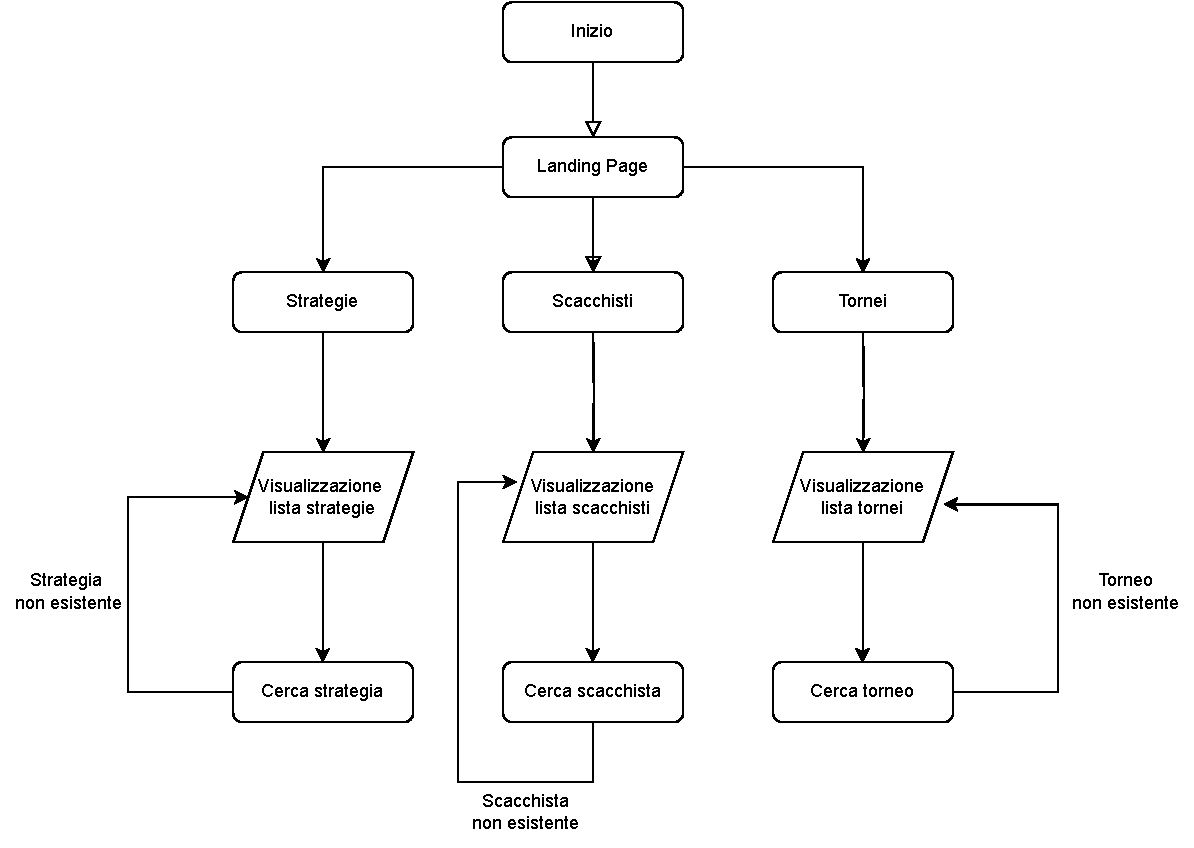
\includegraphics[scale=.8]{~/studio/uni/corsi_22_23/modsem/progetto/relazione/FlussoMODSEM2023.drawio.pdf}
\end{figure}

\begin{figure}[h]
  \caption{Mockup della landing page del sito.}
  \centering
  \label{fig:landing}
  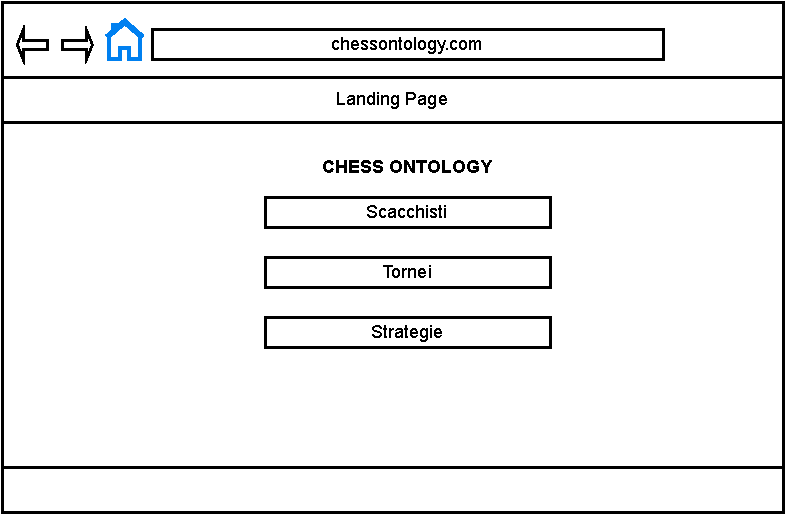
\includegraphics[scale=1]{~/studio/uni/corsi_22_23/modsem/progetto/relazione/landingpage.drawio.pdf}
\end{figure} 

\begin{figure}[h]
  \caption{Mockup della pagina specifica per gli scacchisti del sito.}
  \centering
\label{fig:scacchisti}
  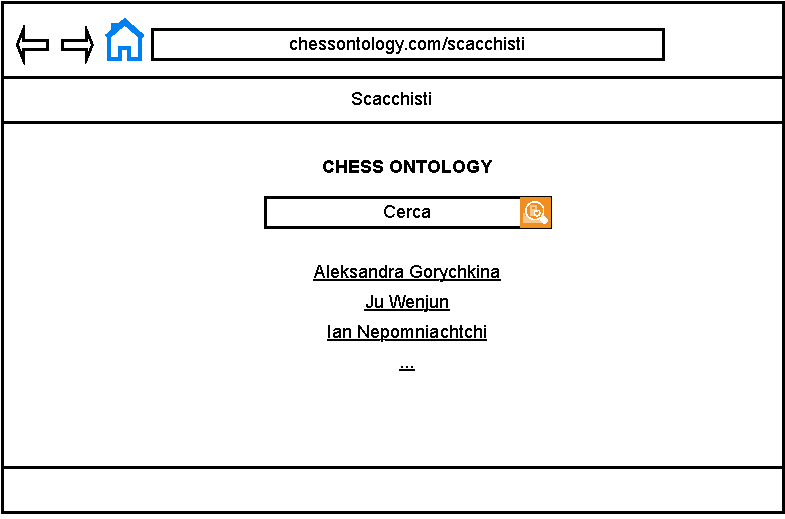
\includegraphics[scale=1]{~/studio/uni/corsi_22_23/modsem/progetto/relazione/scacchisti.drawio.pdf}
\end{figure} 

\begin{figure}[h]
  \caption{Mockup della pagina specifica per le strategie del sito.}
  \centering
\label{fig:strategie}
  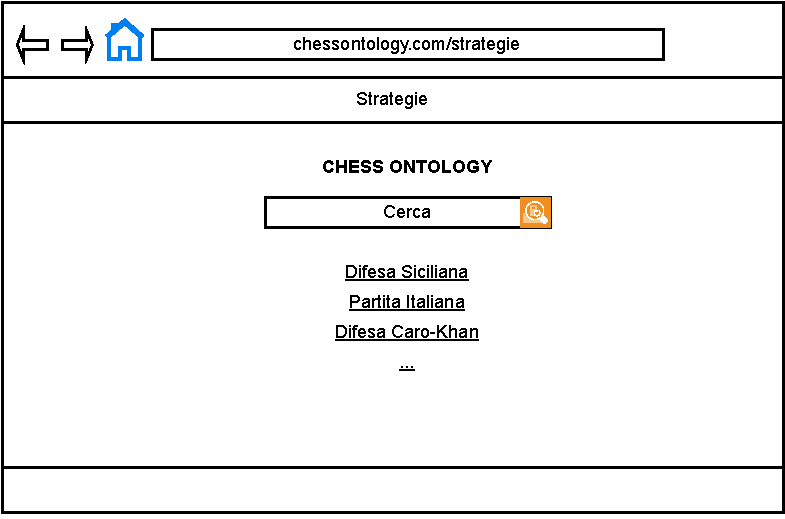
\includegraphics[scale=1]{~/studio/uni/corsi_22_23/modsem/progetto/relazione/strategie.drawio.pdf}
\end{figure} 


\begin{figure}[h]
  \caption{Mockup della pagina specifica per i tornei del sito.}
  \centering
\label{fig:tornei}
  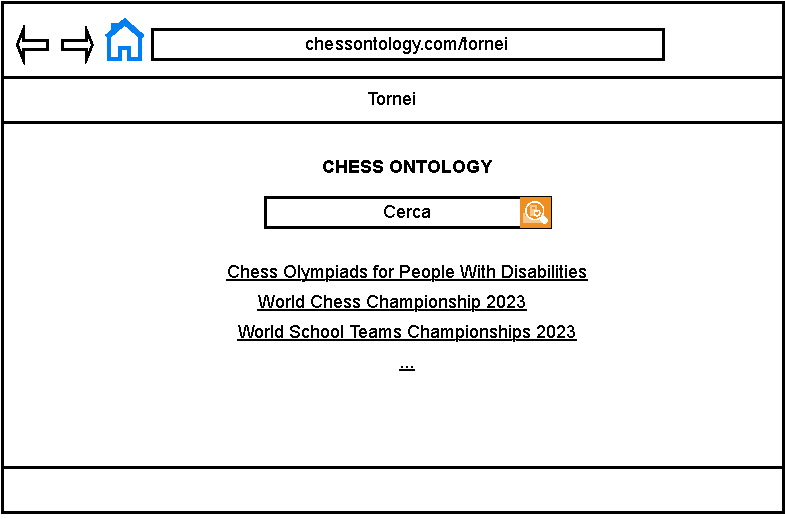
\includegraphics[scale=1]{~/studio/uni/corsi_22_23/modsem/progetto/relazione/tornei.drawio.pdf}
\end{figure} 

\chapter{Query SPARQL}

\section{1 - Quali sono le principali strategie scacchistiche considerate
\textit{aggressive}?}

\begin{verbatim}
PREFIX owl: <http://www.w3.org/2002/07/owl#>
PREFIX rdf: <http://www.w3.org/1999/02/22-rdf-syntax-ns#>
PREFIX rdfs: <http://www.w3.org/2000/01/rdf-schema#>
PREFIX scacchi: <http://www.semanticweb.org/leno/ontologies/2023/11/scacchi2023#>

SELECT ?strategia
WHERE {
    ?strategia rdf:type scacchi:StrategiaAggressiva.
}
\end{verbatim}

Questa query permette di ottenere informazioni riguardo tutte le
istanze della classe \textit{StrategiaAggressiva}, quindi tutte le
aperture che in generale sono prone a generare una partita con molti
cambi. Sono strategie diametralmente opposte e mutualmente esclusive a
quelle di Posizione, della classe \textit{StrategiaDiPosizione}. Il
fatto che siano mutualmente esclusive viene riportato nell'ongologia
tramite un legame \textit{disjointWith}.

I dati ottenuti da tale query sono mostrati in figura \ref{fig:query1}.

\begin{figure}[h]
  \caption{Risultati della query 1.}
  \centering
  \label{fig:query1}
  \includegraphics[scale=1]{~/Pictures/Screenshots/Screenshot_20240104_174014.png}
\end{figure} 

\section{2 - Quante partite ha vinto 'Ding Liren'?}

\begin{verbatim}
PREFIX owl: <http://www.w3.org/2002/07/owl#>
PREFIX rdf: <http://www.w3.org/1999/02/22-rdf-syntax-ns#>
PREFIX rdfs: <http://www.w3.org/2000/01/rdf-schema#>
PREFIX scacchi: <http://www.semanticweb.org/leno/ontologies/2023/11/scacchi2023#>

SELECT (COUNT(?partitevinte) AS ?numeroPartiteVinte)
WHERE {
    scacchi:DingLiren scacchi:vincitorePartita ?partitevinte.
}
\end{verbatim}

Questa query è generalmente utile per ottenere informazioni riguardo
il numero di vittorie ottenute da uno specifico giocatore. Sicuramente
è una delle query più popolari e frequenti, sia per curiosità degli
utenti, ma anche per quelle che possono essere query automatiche
scritte con il fine di costruire statistiche sui vari giocatori, e
mantenere le pagine informative relative ad essi sempre aggiornate.

I dati ottenuti da tale query sono mostrati in figura \ref{fig:query2}.
Essendo presente nell'ontologia un'unica partita vinta da Ding Liren,
viene conteggiata solo essa.

\begin{figure}[h]
  \caption{Risultati della query 2.}
  \centering
  \label{fig:query2}
  \includegraphics[scale=1]{~/Pictures/Screenshots/Screenshot_20240104_174230.png}
\end{figure} 

\section{3 - Chi è stato l'ultimo vincitore del torneo Chess Olimpyads For
People with Disabilities?}

\begin{verbatim}
PREFIX owl: <http://www.w3.org/2002/07/owl#>
PREFIX rdf: <http://www.w3.org/1999/02/22-rdf-syntax-ns#>
PREFIX rdfs: <http://www.w3.org/2000/01/rdf-schema#>
PREFIX scacchi: <http://www.semanticweb.org/leno/ontologies/2023/11/scacchi2023#>

SELECT ?winnername
WHERE {
  ?x scacchi:vincitoreTorneo scacchi:ChessOlympiadsForPeopleWithDisabilities2023.
  ?x scacchi:nomeCompleto ?winnername.
}
\end{verbatim}

Questa query è utile per ottenere informazioni riguardo l'ultimo
vincitore di uno specifico torneo, in questo caso si tratta del torneo
\textit{Chess Olimpyads For People With Disabilities} del 2023. Anche
in questo caso, è una query molto importante e certamente molto
frequente, perchè è un informazione che può essere utile per diversi
scopi, primo fra tutti quello educativo, ma anche per scopi di analisi
e raccolta dati.

I dati ottenuti da tale query sono mostrati in figura \ref{fig:query3}.

\begin{figure}[h]
  \caption{Risultati della query 3.}
  \centering
  \label{fig:query3}
  \includegraphics[scale=1]{~/Pictures/Screenshots/Screenshot_20240104_174642.png}
\end{figure} 

\section{4 - Quale giocatore ha vinto più partite usando la difesa siciliana?}

\begin{verbatim}
PREFIX owl: <http://www.w3.org/2002/07/owl#>
PREFIX rdf: <http://www.w3.org/1999/02/22-rdf-syntax-ns#>
PREFIX rdfs: <http://www.w3.org/2000/01/rdf-schema#>
PREFIX scacchi: <http://www.semanticweb.org/leno/ontologies/2023/11/scacchi2023#>

SELECT ?x (COUNT(?partitevinte) AS ?numeroPartiteVinte)
WHERE {
  ?x scacchi:vincitorePartita ?partitevinte.
    scacchi:difesaSiciliana scacchi:strategiaPartitaNero ?partitevinte.
}
GROUP BY ?x
ORDER BY ASC(?numeroPartiteVinte)
\end{verbatim}

L'obiettivo centrale di questa query è più specifica per l'ambito
statistico, ovvero cercare di capire quale giocatore favorisce una
certa strategia, e quante volte tale strategia è stata motivo di
vittoria per tale giocatore. Questo genere di informazione, talvolta
più avanzata e specifica rispetto a quelle estratte dalle query
precedenti, può certamente tornare utile anche ai giocatori più
esperti, per apprendere ed imitare lo stile di gioco dei
professionisti.

I dati ottenuti da tale query sono mostrati in figura \ref{fig:query4}.

\begin{figure}[h]
  \caption{Risultati della query 4.}
  \centering
  \label{fig:query4}
  \includegraphics[scale=.65]{~/Pictures/Screenshots/Screenshot_20240104_175016.png}
\end{figure} 

\section{5 - Chi è la/lo scacchista con il punteggio Elo più alto?}

\begin{verbatim}
PREFIX owl: <http://www.w3.org/2002/07/owl#>
PREFIX rdf: <http://www.w3.org/1999/02/22-rdf-syntax-ns#>
PREFIX rdfs: <http://www.w3.org/2000/01/rdf-schema#>
PREFIX scacchi: <http://www.semanticweb.org/leno/ontologies/2023/11/scacchi2023#>

SELECT ?giocatore ?punteggio
WHERE {
    ?giocatore rdf:type scacchi:Scacchista.
    ?giocatore scacchi:punteggioElo ?punteggio.
}
ORDER BY DESC(?punteggio)
\end{verbatim}

Anche questa query sarà certamente fra le più frequenti, se non la più
frequente. Certamente l'attenzione generale sarà sempre rivolta alle
personalità che dominano i rispettivi campi. Essendo il punteggio Elo
la metrica con cui viene valutata la bontà di una/uno scacchista,
certamente sarà uno dei dati più richiesti.

I dati ottenuti da tale query sono mostrati in figura \ref{fig:query5}.

\begin{figure}[h]
  \caption{Risultati della query 5.}
  \centering
  \label{fig:query5}
  \includegraphics[scale=.8]{~/Pictures/Screenshots/Screenshot_20240104_175302.png}
\end{figure} 


\chapter{Regole SWRL}

Come estensione a scelta, ho scelto la scrittura di regole $SWRL$, che
permettano di inferire informazioni ulteriori a quelle ottenibili dal
reasoner presente in Protegè.
Seguono le regole swirl con relativa giustificazione.

\section{Regola 1}

Aggiungo alla sottoclasse $Scacchista$ una classe
$ScacchistaVittoriosu$ (niente typo, vedi disclaimer), in cui inserire tutte le istanze della classe
scacchista che abbiano vinto almeno una partita.
La regola è definita come segue:
\begin{verbatim}

scacchi2023:Scacchista(?x) ^ scacchi2023:vincitorePartita(?x, ?y) 
      -> scacchi2023:ScacchistaVittoriosu(?x)

\end{verbatim}

\section{Regola 2}

È stata aggiunta la sottoclasse $WorldChampion$ alla classe
$ScacchistaProfessionista$, con il fine di identificare tutti le/gli
scacchisti che abbiano vinto almeno un campionato del mondo, ovvero
un torneo ufficiale internazionale appartenente alla classe
$WorldChampionship$, sottoclasse di $TorneoInternazionale$.

\newpage

\begin{verbatim}

scacchi2023:ScacchistaProfessionista(?x) ^ scacchi2023:WorldChampionship(?t) 
^ scacchi2023:vincitoreTorneo(?x, ?t) -> scacchi2023:WorldChampion(?x)

\end{verbatim}

\section{Regola 3}

La presente regola, e le successive due, hanno lo scopo di
categorizzare secondo i ranking e rating ufficiali della FIDE, tutti
le/gli scacchiste/i professioniste/i, in relazione al loro punteggio ELO.
Abbiamo infatti, secondo regolamento ufficiale, che:
\begin{itemize}
  \item Professioniste/i con punteggio ELO superiore ai 2300 sono
    classificate/i come \textit{Mestri FIDE}, nell'ontologia
    identificate/i nella classe $FM$
  \item Professioniste/i con punteggio ELO superiore ai 2400 sono
    classificati come \textit{Mestri Internazionali}, nell'ontologia
    identificati nella classe $IM$
  \item Professioniste/i con punteggio ELO superiore ai 2500 sono
    classificati come \textit{Granmestri}, nell'ontologia
    identificati nella classe $GM$
\end{itemize}

\begin{verbatim}
scacchi2023:ScacchistaProfessionista(?x) ^
scacchi2023:punteggioElo(?x, ?punteggio) ^
swrlb:greaterThan(?punteggio, 2300) -> scacchi2023:FM(?x)
\end{verbatim}

\section{Regola 4}

Maestro Internazionale

\begin{verbatim}
scacchi2023:ScacchistaProfessionista(?x) ^
scacchi2023:punteggioElo(?x, ?punteggio) ^
swrlb:greaterThan(?punteggio, 2400) -> scacchi2023:IM(?x)
\end{verbatim}

\section{Regola 5}

Gran Maestro

\begin{verbatim}
scacchi2023:ScacchistaProfessionista(?x) ^
scacchi2023:punteggioElo(?x, ?punteggio) ^
swrlb:greaterThan(?punteggio, 2500) -> scacchi2023:GM(?x)
\end{verbatim}

\end{document}
